% Borg GPU — HPG 2026 Poster
% A0 portrait, tikzposter  (HPG 2026 requires portrait)

\documentclass[a0paper,portrait,20pt]{tikzposter}

% ── Theme ──────────────────────────────────────────────────────────────────
\usetheme{Simple}
\useblockstyle{Basic}

% ── Teal palette ───────────────────────────────────────────────────────────
\definecolorstyle{Mono}{
  \definecolor{monoDeep}{HTML}{082830}   % near-black teal
  \definecolor{monoDark}{HTML}{085868}   % dark teal
  \definecolor{monoMid} {HTML}{2E6878}   % mid teal
  \definecolor{monoLight}{HTML}{C8E8E8}  % very pale teal
  \definecolor{vkbg}    {HTML}{FFFFFF}   % white background (print-friendly)
}{
  \colorlet{backgroundcolor}{vkbg}
  \colorlet{framecolor}{black}
  \colorlet{titlebgcolor}{monoDark}
  \colorlet{titlefgcolor}{white}
  \colorlet{blocktitlebgcolor}{monoDark}
  \colorlet{blocktitlefgcolor}{white}
  \colorlet{blockbodybgcolor}{monoLight}
  \colorlet{blockbodyfgcolor}{black}
  \colorlet{innerblocktitlebgcolor}{monoMid}
  \colorlet{innerblocktitlefgcolor}{white}
  \colorlet{innerblockbodybgcolor}{monoLight}
  \colorlet{innerblockbodyfgcolor}{black}
  \colorlet{notebgcolor}{monoLight}
  \colorlet{notefgcolor}{monoDeep}
  \colorlet{notefrcolor}{black}
}
\usecolorstyle{Mono}

% ── Packages ───────────────────────────────────────────────────────────────
\usepackage[utf8]{inputenc}
\usepackage[T1]{fontenc}
\usepackage{lmodern}
\usepackage{booktabs}
\usepackage{graphicx}
\usepackage{tikz}
\usetikzlibrary{positioning}
\usepackage{amsmath,amssymb}
\usepackage{xcolor}
\usepackage{enumitem}
\usepackage{url}
\usepackage[final]{qrcode}
\newcommand{\todo}[1]{\textcolor{red}{[#1]}}

% ── Custom colours ─────────────────────────────────────────────────────────
\definecolor{borgblue}{HTML}{085868}
\definecolor{borgorange}{HTML}{E87722}
\definecolor{borggreen}{HTML}{1A9080}

% ── Helpers ────────────────────────────────────────────────────────────────
\newcommand{\done}{\textcolor{borggreen}{$\checkmark$}}
\newcommand{\inprog}{{\textcolor{monoMid}{\textbf{[wip]}}}}

% ── Title ──────────────────────────────────────────────────────────────────
\title{\parbox{0.85\linewidth}{\centering \textbf{Borg} (\textbf{B}ring yer \textbf{O}wn \textbf{G}Raphics): \\
  An Open-Source Tile-Based GPU with Silicon Tapeout}}
\author{Andreas Wendleder}
\institute{Independent Researcher, Landshut, Germany
           \quad \texttt{andreas.wendleder@proton.me}
           \quad \texttt{github.com/gonsolo/Borg}
           \quad \texttt{orcid.org/0009-0008-8304-2818}}
\date{HPG 2026, July 17--19, Los Angeles, CA}

\makeatletter
\settitle{ \vbox{ \centering
  \color{titlefgcolor} {\bfseries \Huge \@title \par}
  \vspace*{1em}
  {\huge \@author \par} \vspace*{0.5em}
  {\Large \@institute \par} \vspace*{0.5em}
  {\Large \@date \par}
} }
\makeatother

% ══════════════════════════════════════════════════════════════════════════
\begin{document}
\maketitle[titletotopverticalspace=4cm, titleverticalspace=2cm]

% ── Full-width SoC diagram (outside columns) ──────────────────────────────
\block{SoC \& TBDR Architecture}{
Borg is a complete \textbf{RISC-V SoC} featuring the \textbf{Hutt} core.
The GPU follows the Tile-Based Deferred Rendering paradigm:

\medskip
\begin{center}
  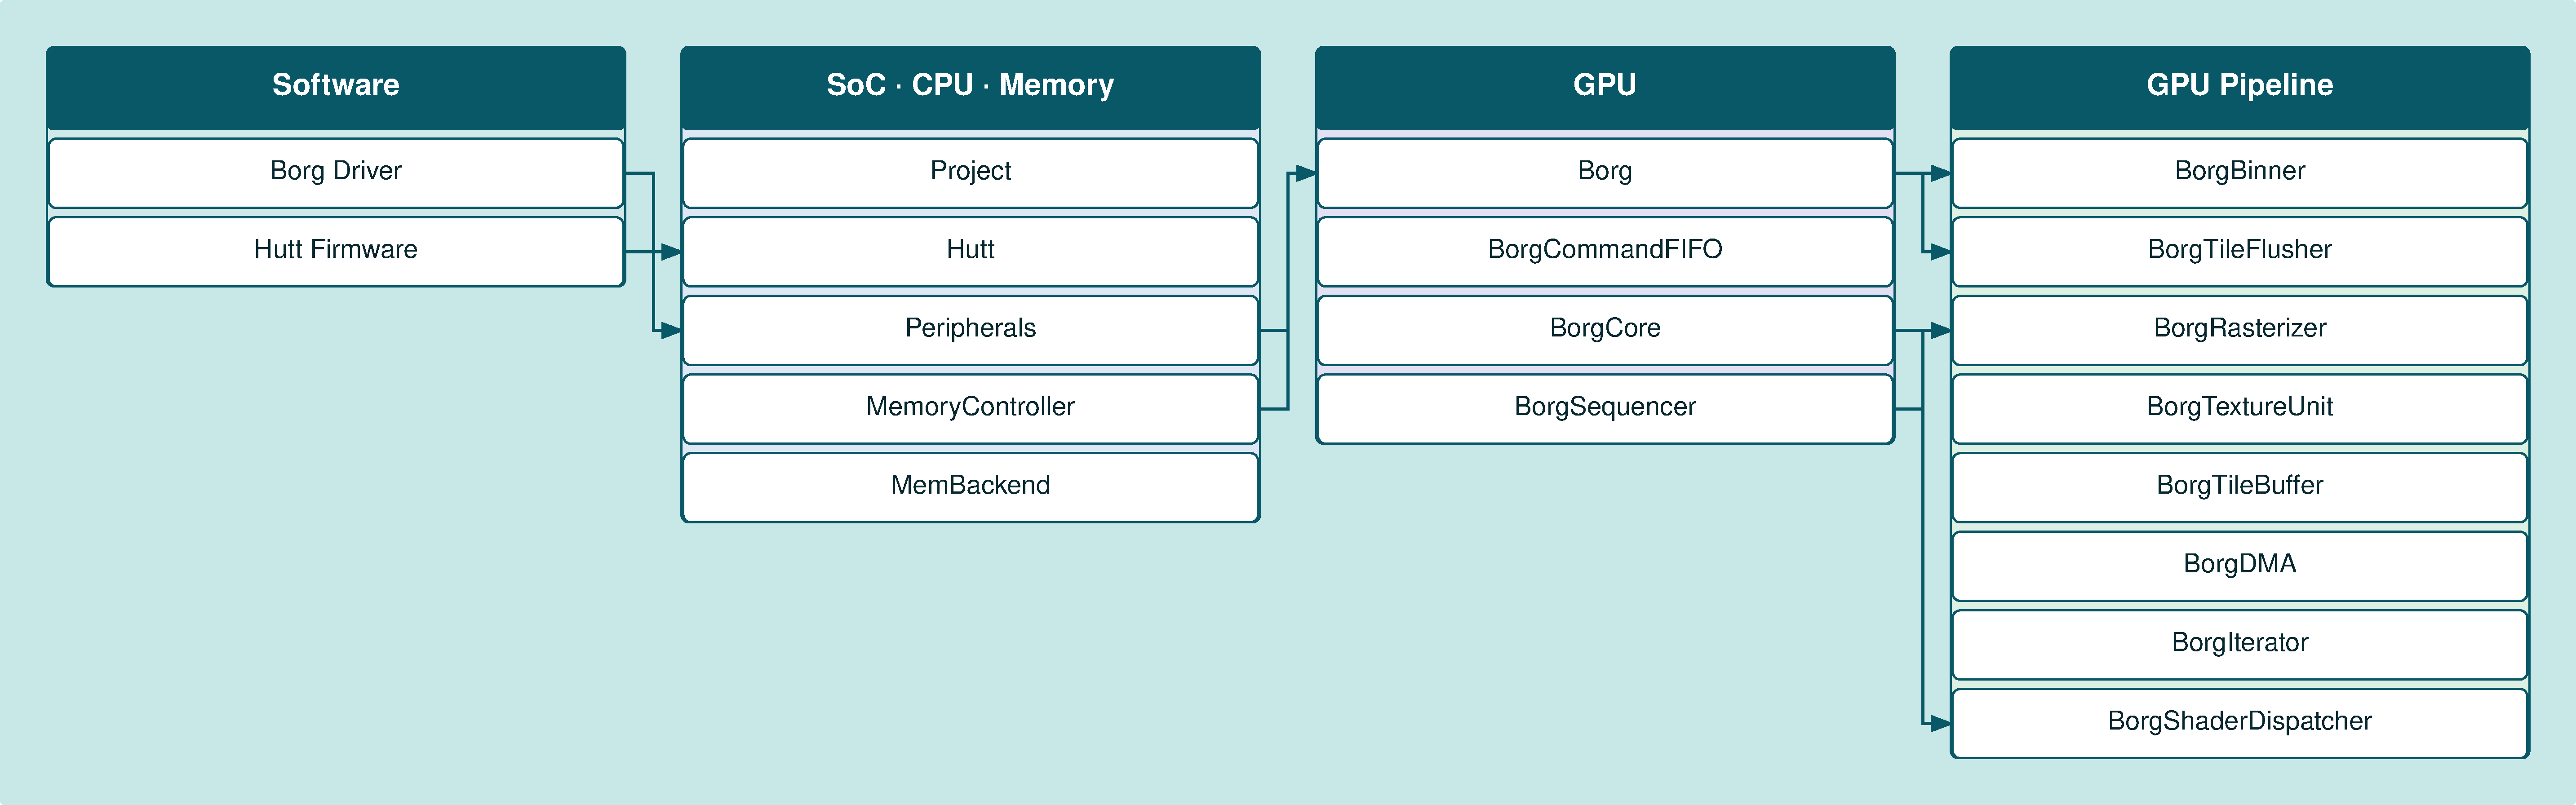
\includegraphics[width=0.96\linewidth]{hw_diagram}
\end{center}

\medskip
Geometry is binned tile-by-tile; shaded fragments are written to an
on-chip tile buffer (4$\times$4 pixels, FP16 RGBZ), minimising external memory bandwidth.
The tile buffer is flushed to SDRAM only after all triangles covering that tile are rendered.
}

% ── Three columns below the SoC diagram ───────────────────────────────────
\begin{columns}

% ════════════════════════════════
%  COLUMN 1
% ════════════════════════════════
\column{0.333}

\block{Motivation}{
\begin{itemize}[leftmargin=*,nosep]
  \item Every commercial GPU hides its microarchitecture behind NDAs
  \item This blocks \textbf{reproducibility}, \textbf{teaching}, and
        architectural experiments
  \item \textbf{Concise:} Hardware (\textbf{1513 LoC} Scala), Compiler
        (\textbf{1600 LoC} Python), Firmware (\textbf{2000 LoC} C).
        Total stack \textbf{< 6k lines}.
  \item Open GPU simulators exist — but \emph{no open GPU has reached silicon}
\end{itemize}

\medskip
\textbf{Borg} is the fully open answer: a TBDR GPU \textbf{SoC} in Chisel,
built with an open toolchain, and \textbf{submitted for ASIC tapeout}.
Borg has contributed \textbf{68 patches upstream} to the open EDA ecosystem.

\medskip
\begin{center}
{\large\textcolor{borgorange}{\textbf{To our knowledge: the only open-source\\
GPU with a submitted ASIC tapeout.}}}
\end{center}
}

\block{Current Demo}{
Running on \textbf{ULX3S} (ECP5-85K) with \textbf{HDMI output}:
\begin{itemize}[leftmargin=*,nosep]
  \item 12 textured triangles, 128$\times$128 framebuffer, double-buffered
  \item Full pipeline: vertex shader $\to$ texture fetch $\to$ Z-buffer $\to$ HDMI
  \item Orchestrated by integrated \textbf{Hutt} RISC-V core
\end{itemize}
\medskip
\begin{center}
  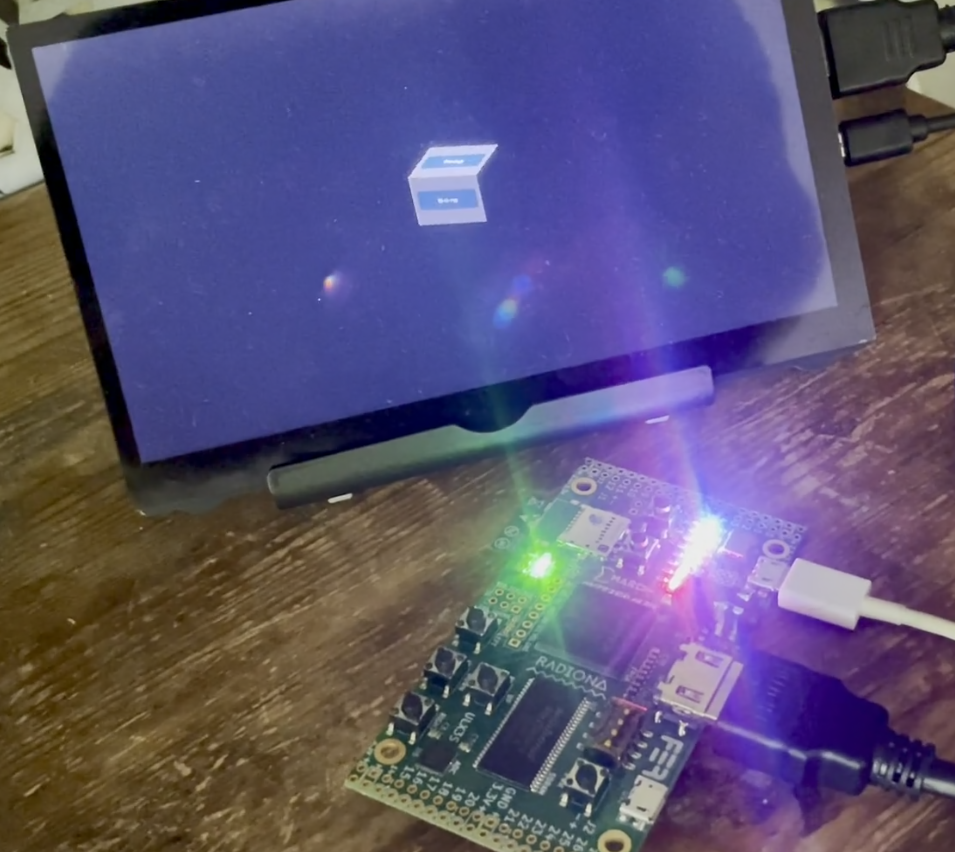
\includegraphics[width=0.55\linewidth]{ulx3s_vkcube}\\[0.4em]
  {\small\itshape VkCube running on ULX3S hardware with HDMI output}
\end{center}
}

\block{ASIC Tapeouts (Tiny Tapeout)}{
\centering \small
\begin{tabular}{@{}llllr@{}}
\toprule
\textbf{Run} & \textbf{Process} & \textbf{Tiles} & \textbf{Content} & \textbf{Cost} \\
\midrule
TTIHP26a & IHP 130\,nm  & 8 tiles  & FP peripheral & 515\,€ \\
\bottomrule
\end{tabular}

\medskip
\centering
Submitted; chips expected September 2026.
}

\block{Funding}{
\begin{center}

\includegraphics[height=2.2cm]{figures/nlnet_logo}
\qquad

\includegraphics[height=2.2cm]{figures/ngi0_logo}
\end{center}
\medskip
\footnotesize
Borg is funded by the \textbf{NGI0 Commons Fund} (NLnet Foundation /
European Commission, Grant No.~101135429) and Swiss SERI.
}

% ════════════════════════════════
%  COLUMN 2
% ════════════════════════════════
\column{0.333}

\block{Development Roadmap: Phases 1--6}{
\begin{itemize}[leftmargin=*,nosep]
  \item \textbf{Phase 1} \done\ — \textbf{Foundational Architecture} (2025)
  \item \textbf{Phase 2} \done\ — \textbf{GPU Autonomy / 28-Day Sprint}
  \item \textbf{Phase 3} — \textbf{Linux-Capable CPU} (M/A/MMU)
  \item \textbf{Phase 4} — \textbf{Mesa Vulkan Driver} (NIR $\to$ SPIR-B)
  \item \textbf{Phase 5} — \textbf{Hardware Extensions} (SIMD, Blending)
  \item \textbf{Phase 6} — \textbf{Vulkan 1.0 Conformance}
\end{itemize}

\medskip
\centering
\begin{tabular}{@{}cl@{}}
\toprule
\textbf{Status} & \textbf{Key Phase 2 Milestones} \\
\midrule
\done & 32-bit RISC-V ISA + Perspective Proj.\ \\
\done & Triangle Clipping + Fragment Interpolation \\
\done & Pixel Iterator (Rasterizer) + Z-Buffer \\
\done & Command FIFO + SystemRDL Register Map \\
\done & Texture Fetch + Shared Memory Controller \\
\done & GPU DMA Engine + Vertex Sequencer \\
\bottomrule
\end{tabular}
}

\block{Open-Source Toolchain}{
\centering
\begin{tabular}{@{}ll@{}}
\textbf{HDL}        & Chisel (Scala, \textbf{1513 lines}) \\
\textbf{Synthesis}  & Yosys \\
\textbf{P\&R}       & nextpnr-ecp5 / \textbf{LibreLane} (Nix) \\
\textbf{Simulation} & Verilator, cocotb, Arcilator \\
\textbf{Compiler}   & SPIR-V $\to$ SPIR-B (\textbf{1600 lines} Python) \\
\textbf{Firmware}   & 32-bit RISC-V (\textbf{2000 lines} C) \\
\textbf{Reg.\ map}  & PeakRDL-chisel \\
\textbf{Math Cores} & \textbf{Berkeley Hardfloat} (FMA) \\
\textbf{PDKs}       & sky130A, gf180mcuD, ihp-sg13g2 \\
\end{tabular}

\medskip
\centering
\textbf{Reproducible Build:} \texttt{direnv} + \textbf{Nix} flakes. \\
Zero-install setup for all 18+ EDA tools. \\
\textbf{Ecosystem Impact:} Pioneers the first fully reproducible ASIC flow
in \texttt{nixpkgs} (LibreLane merged Jan 2026).
}

\block{Comparison with Related Open GPUs}{
\centering
\begin{tabular}{@{}l@{\hskip 0.5em}c@{\hskip 0.5em}c@{\hskip 0.5em}c@{}}
\toprule
& \textbf{Borg} & \textbf{Nyuzi} & \textbf{Vortex} \\
\midrule
Architecture    & TBDR    & GPGPU   & RISC-V GPGPU \\
ISA             & Custom  & Custom  & RV32\\
Tapeout         & submitted & —       & — \\
Open toolchain  & \done   & partial & partial \\
Target          & ECP5    & Arria 5 & Xilinx \\
\bottomrule
\end{tabular}
}

\block{Design Values}{
\begin{description}[leftmargin=*,nosep]
  \item[Transparency] No binary blobs, no hidden firmware.
  \item[Accessibility] Runs on a \$20 FPGA; uses \$500 ASIC runs.
  \item[Simplicity] Minimalist TBDR pipeline for maximum performance/area.
\end{description}
}

% ════════════════════════════════
%  COLUMN 3
% ════════════════════════════════
\column{0.333}

\block{Future Work \& Open Questions}{
\begin{itemize}[leftmargin=*,nosep]
  \item \textbf{800$\times$480 HDMI} native resolution (DDC/EDID)
  \item Higher fps via SDRAM burst writes and uniform caching
  \item SIMD-2 FMA for 2$\times$ fragment shader throughput
  \item BVH ray traversal ISA extensions (path tracing)
\end{itemize}
\medskip
\textbf{Open questions:}
\begin{itemize}[leftmargin=*,nosep]
  \item Can a TBDR pipeline scale to multi-core tiles?
  \item Minimal ISA for hardware BVH traversal?
  \item How to best expose Borg via Mesa Vulkan?
\end{itemize}
}

\block{The Transparency Gap: Borg vs.\ Commercial}{
\centering \small
\begin{tabular}{@{}lccc@{}}
\toprule
\textbf{Feature} & \textbf{Borg} & \textbf{Mobile} & \textbf{Desktop} \\
\midrule
RTL Source       & \textbf{Open}   & Proprietary & Proprietary \\
EDA Toolchain    & \textbf{Libre}  & Proprietary & Proprietary \\
Silicon Layout   & \textbf{Public} & Secret      & Secret \\
ISA Specs        & \textbf{Public} & Often NDA   & Proprietary \\
\bottomrule
\end{tabular}

\medskip
\centering \normalsize
\textbf{Borg} is the only design where researchers can
inspect the layout and modify logic without NDAs.
}

\block{Physical Design (GDSII)}{
  \begin{center}
    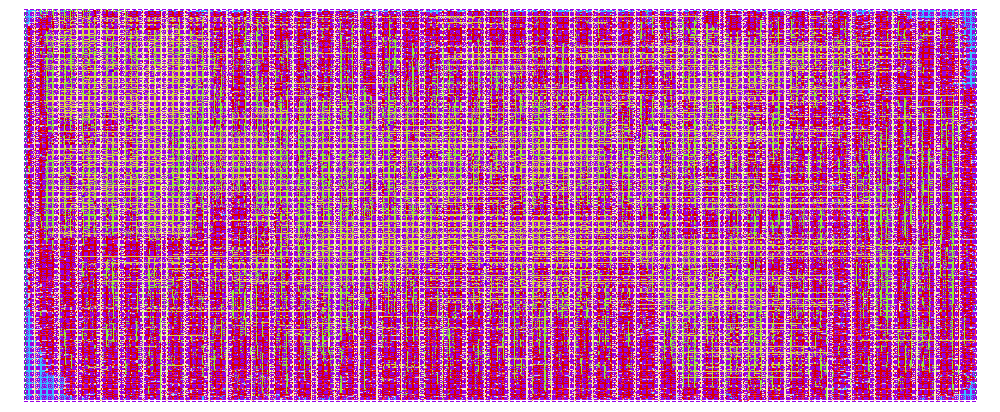
\includegraphics[width=0.95\linewidth]{gds_render_small}
  \end{center}
  \centering \small
  \begin{tabular}{@{}ll@{}}
  \toprule
  \textbf{Metric} & \textbf{Value (TTIHP26a)} \\
  \midrule
  Logic Area      & $0.95 \times 0.95$\,mm (8 tiles) \\
  Est.\ Gate Count & $\sim$90k (excl.\ BRAM) \\
  Clock Target    & 50\,MHz (Standard Cell) \\
  \bottomrule
  \end{tabular}
}

\block{Selected References \& Learn More}{
\footnotesize
\begin{enumerate}[leftmargin=1.5em,nosep,label={[\arabic*]}]
  \item \textbf{M. Bell}, \emph{TinyQV: A RISC-V Core for Tiny Tapeout}, 2024.
  \item \textbf{J. Bush}, \emph{Nyuzi Parallel Processor}, GPGPU-7, 2014.
  \item \textbf{A. Taneja et al.}, \emph{Vortex: Open Source RISC-V GPGPU}, 2021.
  \item \textbf{Bachrach et al.}, \emph{Chisel: HW in a Scala DSL}, DAC 2012.
  \item \textbf{C. Wolf}, \emph{Yosys Open SYnthesis Suite}, 2012.
  \item \textbf{M. Venn}, \emph{Tiny Tapeout: Open Access Silicon}, 2023.
  \item \textbf{A. Wendleder}, \emph{LibreLane in nixpkgs}, PR \#471712, 2026.
\end{enumerate}
\smallskip
\begin{center}
\begin{minipage}{0.45\linewidth}
  \centering
  \qrcode[height=3cm]{https://github.com/gonsolo/Borg}\\[0.2em]
  {\small\textbf{Source Code}}
\end{minipage}
\hfill
\begin{minipage}{0.45\linewidth}
  \centering
  \qrcode[height=3cm]{https://gonsolo.github.io/Borg}\\[0.2em]
  {\small\textbf{Book / Docs}}
\end{minipage}
\end{center}
\smallskip
\centering \footnotesize \texttt{andreas.wendleder@proton.me}
}

\end{columns}

\end{document}
